%===================================================================================================
\subsection{Sex Work: Population Sizes \& Partner Numbers}\label{model.par.sw}
%---------------------------------------------------------------------------------------------------
\subsubsection{Population Sizes}\label{model.par.sw.size}
Population sizes of all activity groups are modelled as proportions of the total population,
which are assumed to remain roughly constant.
Individuals can, however, move between groups (see \sref{model.par.turn.act})
--- \ie groups are open populations ---
and disproportionate mortality due to HIV between groups
may cause higher risk groups to shrink over time.
%---------------------------------------------------------------------------------------------------
\paragraph{Female Sex Workers}
The proportion of women who report sex work in national demographic and health surveys
is generally considered unreliable due to social desirability bias,
particularly if the survey is face-to-face and household-based
\cite{Konings1995,Gregson2002,Gregson2004,Lowndes2012,Behanzin2013}.
Therefore, FSW population size estimates require
targeted surveys and unique methodologies \cite{UNAIDS2010kps,Abdul-Quader2014}.
In both \cite{EswKP2014} and \cite{EswIBBS2022}, the Swati FSW population size
was estimated using a combination of
unique object method, service multiplier method, prior survey participation,
and network scale-up method (NSUM) \cite{UNAIDS2010kps}.
In 2011 \cite{EswKP2014}, regional FSW population size estimates
ranged from 0.7\% to 6.5\% of all women,
with overall population-weighted mean across regions of 2.9\%;
in 2021 \cite{EswIBBS2022}, the mean (95\%~CI) estimates were 2.43~(1.17,~5.02)\%.
To reflect this uncertainty in the model, a BAB distribution was fitted
such that 95\% of the probability fell between 0.7\% and 6.5\%,
and used as the prior distribution for the proportion of women who are FSW:
$P_{s_{1}i_{34}} / P_{s_{1}}$.
Then, following the analysis in \sref{model.par.fsw},
the proportion of all FSW in the higher risk FSW group was fixed at 20\%,
and likewise the lower risk group at 80\%.
%---------------------------------------------------------------------------------------------------
\paragraph{Clients of FSW}
Similar to FSW, household-based surveys are not considered reliable data sources
for estimating the population size of clients of FSW \cite{Behanzin2013}.
However, few surveys are designed to reach clients of FSW,
and no direct estimates of FSW size exist for Eswatini.
So, I use a common approach for inferring the FSW client size \cite{Cote2004},
similar to the ``multiplier method'' \cite{Morison2001}.
Given the FSW population proportion $P_{s_{1}i_{34}}$,
the number of average yearly new and regular sex work clients per FSW $Q_{p_{34}s_{1}i_{34}}$,
the frequency of sex per partnership-year $F_{p_{34}}$, and
the total number of yearly commercial sex acts per client year $Q_{p_{34}s_{2}i_{34}}\,F_{p_{34}}$,
the total client population $P_{s_{2}i_{34}}$ is defined as:
\begin{equation}
  {\textstyle\sum_{i}} P_{s_{2}i_{34}} =
  \frac{\sum_{pi} P_{s_{1}i}\,Q_{p_{34}s_{1}i_{34}}\,F_{p_{34}}}
       {\sum_{pi}             Q_{p_{34}s_{2}i_{34}}\,F_{p_{34}}}
  \label{eq:model.fsw.cli.tot}
\end{equation}
Then, as with FSW, the proportion of total clients in the higher risk client group
is defined as 20\% of all clients, and likewise for the lower risk group at 80\%.
Using $Q_{p_{34}s_{1}i_{34}}$, $Q_{p_{34}s_{2}i_{34}}$, and $F_{p_{34}}$
as defined below in \sref{model.par.sw.part}, the client population size $P_{s_{2}i_{34}}$
estimated by this method was 14.5~(5.2,~33.9)\% of men.
%---------------------------------------------------------------------------------------------------
\subsubsection{Sex Work Partnerships}\label{model.par.sw.part}
%---------------------------------------------------------------------------------------------------
\paragraph{Female Sex Workers}
Table~\ref{tab:fsw.ratios} summarizes
the numbers of new and regular clients \emph{per month} reported by Swati FSW,
stratified by higher \vs lower risk per the analysis in \sref{model.par.fsw.fac}.
In general, the numbers of partners ``$C$'' reported
for a given recall period $\gamma$ (\eg 1 month)
do not directly inform a partnership formation rate $Q$ nor a number of concurrent partners $K$
(see \sref{app.model.math.qp});
rather, under certain assumptions, $Q$ and $K$ can be defined as:
\begin{alignat}{1}
  Q &= \frac{C}{\gamma+\delta} \label{eq:C2Q}\\
  K &= \frac{C\delta}{\gamma+\delta} = Q\delta \label{eq:C2K}
\end{alignat}
The choice of force of infection model (see Chapter~\ref{foi})
will determine whether $Q$ or $K$ is used.
Moreover, based on the survey questions,%
\footnote{The survey questions were: \shortquote{In the last 30 days,
  how many (new/regular) clients have you had sex with?}, or similar.}
it's not clear whether these reported partner numbers $C$
represent the numbers of unique men or unique client visits.
\par
I assumed that all \emph{new} clients were one-off visits;
thus the reported partner numbers effectively represented
$1/12$th of the total numbers of yearly partnerships $Q_{p_{3}}$.
As such, I sampled the yearly rate of new sex work partnerships among lower risk FSW
from a gamma distribution with mean (95\%~CI) as 4.1~(2.5,~6.0) $\times$ 12,
and the \emph{relative} rate among higher risk FSW from 2.0~(1.6,~2.5).
Since each partnership is assumed to include only one sex act,
the partnership duration $\delta_{p_{3}}$, frequency of sex $F_{p_{3}}$,
and number of concurrent partnerships $K_{p_{3}}$ are ill-defined,
but can be defined for convenience as
$\delta_{p_{3}} = 1/12$ (years), $F_{p_{3}} = 12$ (per year),
and $K_{p_{3}} = Q_{p_{3}} / 12$ (per year).
\par
For \emph{regular} sex work partnerships, uncertainties remain regarding
partnership duration $\delta_{p_{4}}$ (see \sref{model.par.sex.dur}),
frequency of sex per month $F_{p_{4}}/12$, and
survey responses $C$ reflecting unique clients or total client visits per month.
If $C$ reflects the numbers of unique clients, then
$Q_{p_{4}s_{1}i_{34}}$ can be defined via \eqref{eq:C2Q} using $C$ directly;
whereas if $C$ reflects the numbers of unique visits, then
$Q_{p_{4}s_{1}i_{34}}$ should be defined using $C/(F_{p_{4}}/12)$.
I assumed that $\rho = 2/3$ of respondents interpreted the question as in the former case,
and $1-\rho = 1/3$ as in the latter, such that:
\begin{equation}\label{eq:C.swr}
  C' = \rho\,C + (1-\rho)\,C/(F_{p_{4}}/12)
\end{equation}
Taking $F_{p_{4}}/12 = 2$ as the prior mean from \sref{model.par.sex.freq},
\eqref{eq:C.swr} simplifies to $C' = \frac{5}{6}\,C$.
Then, sampling $C_{p_{4}s_{1}i_{3}}$
from a gamma distribution with mean (95\%~CI) 8.4~(6.0,~11.0) from Table~\ref{tab:fsw.ratios},
and $\delta_{p_{4}}$ as specified in \sref{model.par.sex.dur},
I defined $Q_{p_{4}s_{1}i_{3}}$ and $K_{p_{4}s_{1}i_{3}}$
via \eqref{eq:C2Q} using $C'_{p_{4}s_{1}i_{3}}$ and $\gamma = 1/12$ year.
% TODO: (*) summarize distributions: Q, K, KF
For higher risk FSW, I sampled the \emph{relative} number/rate of regular clients from
1.5~(1.3,~1.7) (Table~\ref{tab:fsw.ratios}) as before.
%---------------------------------------------------------------------------------------------------
\paragraph{Clients}
Across Sub-Saharan Africa, data for clients of FSW on
the number of unique FSW visited and the frequency of sex is sparse.
Among 64 clients in Kenya,
the median number of sex work visits per week was 1.3 (68 per year);
most clients (68\%) had 1--3 regular FSW partners simultaneously, and
visited 0--3 new FSW per year \cite{Voeten2002}.
Among 261 truck drivers at sex work hotspots in Uganda,
the mean number of sexual partners was
7.4 in the past 30 days and 44.7 in the past year \cite{Matovu2012}.
\citet{Johnson2017} modelled yearly sex work visits among South African clients of FSW as
gamma-distributed with age over 10, peaking at 64 visits per year for clients aged 37.
To reflect these data, I specified clients overall to have
mean (95\%~CI) 60~(35,~90) sex acts with FSW per year
($K_{p_{34}s_{2}i_{34}}\,F_{p_{34}}/12$, gamma prior).
Then, the yearly sex acts among lower and higher risk clients are defined such that
higher risk have 2.0~(1.6,~2.5) times the number among lower risk.
Finally, since the distribution of sex acts between new \vs regular sex work partnerships
must match that among FSW, the specific values of $K_{p_{34}s_{2}i_{34}}$
were computed automatically.
% TODO: (*) summarize distributions: Q, K, KF
See \sref{model.par.nsw.sw} for numbers of main/spousal and casual partnerships
among FSW and clients.
%===================================================================================================
\subsection{Non-Sex Work: Group Sizes \& Partner Numbers}\label{model.par.nsw}
%---------------------------------------------------------------------------------------------------
\subsubsection{Reported Partner Numbers}\label{model.par.nsw.report}
% TODO: (*) Cockcroft2010
The 2006-07 DHS \cite{SDHS2006}, 2011 SHIMS \cite{SHIMS1}, and 2016-17 SHIMS2 \cite{SHIMS2} surveys
provide the numbers of respondents who reported 2+ partners in the past 12 months (p12m):
13.5, 18.2, 14.5\% among men, and 1.6, 3.8, 4.1\% among women, respectively.%
\footnote{From
  Tables~14.7.1 and 14.7.2 (ages 15-49) in \cite{SDHS2006},
  Table~3 (ages 18-49) in \cite{SHIMS1},
  Table~15.3.A (ages 15+) in \cite{SHIMS2},
  with manual adjustment for survey skip patterns in \cite{SDHS2006,SHIMS2}.}
However, these data do not provide information on the types of partners reported
--- \ie those reporting 1 partner in p12m
are not necessarily in a main/spousal (vs casual) partnership,
and neither are those reporting 2+ partners in p12m.
Moreover, such reports are likely substantially biased by
social desirability bias due to the face-to-face interview format
\cite{Konings1995,Plummer2004,Gregson2004,Behanzin2013}.
\par
Regarding the types of partnerships reported.
Both the 2006 DHS \cite[Tables 14.6.1 and 14.6.2]{SDHS2006}
and 2016-17 SHIMS \cite[Tables 15.4.A and 15.4.B]{SHIMS2}
summarize the numbers of women and men by partners in p12m \emph{and} by marital/union status,
although summaries are stratified by each factor separately, not jointly.
However, making the following assumptions,
I estimated the jointly-stratified proportions of individuals.
Let $W_{2+}$, $W_{1}$, and $W_{0}$ denote women reporting 2+, 1, and 0 partners, respectively,
and likewise with $M_{2+}$, $M_{1}$, $M_{0}$ for men (all partners reflect p12m).%
\footnote{Regarding notation in this section,
  $W_{2+} = P_{s_{1}i_{234}} / P_{s_{1}}$,
  $W_{1} + W_{0} = P_{s_{1}i_{1}} / P_{s_{1}}$, and likewise for men ($M$, $s = 2$).}
The assumptions were:
\begin{itemize}
  \item $W_{2+}$ included all women in non-polygynous unions (married or cohabiting)
  reporting sex with a ``casual'' (non-marital, non-cohabiting) partner
  \item $M_{2+}$ included all men in polygynous unions,
  plus all men in non-polygynous unions reporting sex with a casual partner
  \item the remaining $W_{2+}$ and $M_{2+}$ formed only casual partnerships
  \item all women and men in non-polygynous unions
  reporting no sex with a casual partner reported 1 partner ($W_{1}$ and $M_{1}$)
  \item the remaining $W_{1}$ and $M_{1}$ formed only casual partnerships
\end{itemize}
Figure~\ref{fig:Cwp} illustrates the resulting
proportions of women and men in each union / partners in p12m stratum
in 2006-07 \sfref{fig:Cwp.2006} and 2016-17 \sfref{fig:Cwp.2016}.
\begin{figure}
  \centering
  \begin{subfigure}{0.7\linewidth}
    \centering
    \includegraphics[width=\linewidth]{Cwp.2006}
    \caption{2006-07 \cite{SDHS2006}}
    \label{fig:Cwp.2006}
  \end{subfigure}
  \begin{subfigure}{0.7\linewidth}
    \centering
    \includegraphics[width=\linewidth]{Cwp.2016}
    \caption{2016 \cite{SHIMS2}}
    \label{fig:Cwp.2016}
  \end{subfigure}
  \begin{subfigure}{0.7\linewidth}
    \centering
    \includegraphics[width=\linewidth]{Cwp.adj}
    \caption{Adjusted (mean)}
    \label{fig:Cwp.adj}
  \end{subfigure}
  \caption{Reported proportions of women and men aged 15--49,
    stratified by union status and numbers of partners in the past 12 months}
  \label{fig:Cwp}
\end{figure}
%---------------------------------------------------------------------------------------------------
\paragraph{Reporting Bias}
Next, I consider the issue of reporting bias.
$M_{2+}$ is consistently much greater than $W_{2+}$.
This difference is common in surveys \cite{Todd2009,Higgins2010}, and could be explained by either:
(a) a small number of women with many partners,
such as FSW, who may also not be reached by the survey,
or who may not fully report partner numbers;
(b) over-reporting of partnerships by men; or
(c) under-reporting of partnerships by women.
Further stratification of women reporting 2+ partners in \cite[Table~14.7.1]{SDHS2006}
revealed that 94\% reported exactly 2 whereas 6\% reported 3+,
suggesting that explanation (a) is less likely unless
women with 3+ partners are under-reported or indeed missing from the survey.
\par
\citet{Gregson2002} (Zimbabwe), \citet{Nnko2004} (Tanzania) and \citet{Clark2011} (Kenya)
explored explanations (b) and (c) through measures of consistency; their results suggested that
under-reporting of non-spousal partnerships by women (c) was more likely,
perhaps due to social norms and pressures;
such norms in Eswatini are explored in \cite{Ruark2014,Fielding-Miller2016,Ruark2019,Pulerwitz2021}.
In fact, a review comparing computer-based tools \vs face-to-face interviews
for surveying sexual behaviour \cite{Langhaug2010} found that
\emph{both} women and men may under-report sexual partners, but women more so.
A notable 2008 study in Benin \cite{Behanzin2013} found that
7 times as many married women (21 \vs 3\%) and 3 times as many married men (53 \vs 18\%)
reported any extramarital sex in p12m
in a survey via anonymous polling booth \vs face-to-face interview.
Similarly, 5 times as many unmarried women (13.5 \vs 2.8\%) reported
exchanging sex for money, gifts or favours in p12m, while
4 times as many unmarried men (62 \vs 14\%) reported non-transactional sex with a women in p12m.
Such findings were similar to those from Zimbabwe (1990s) \cite{Gregson2002}.
%---------------------------------------------------------------------------------------------------
\subsubsection{Bias Adjustment: Approach}\label{model.par.nsw.bias}
To account for the above potential reporting biases
and qualitative insights from \cite{Ruark2014,Fielding-Miller2016,Ruark2019,Pulerwitz2021},
I modelled the adjusted proportions of Swati women and men
in each union / partners in p12m stratum as follows.
Let $W_{s1}$ and $W_{u1}$ denote sub-proportions of $W_{1}$ who are single and in a union, respectively,
and likewise for $W_{s2+}$, $W_{u2+}$, $M_{s1}$, $M_{u1}$, $M_{s2+}$, and $M_{u2+}$.
Further, let $W_{s1}$ denote the reported proportion of women (average of 2006-07 and 2016-17),
\vs $W'_{s1}$ denoting the adjusted proportion.
I assumed that a faction of $W_{0}$ belongs in $W'_{s1}$
--- \ie a fraction of women reporting 0 partners in p12m truly had 1 casual (non-main/spousal) partner.
I modelled this relationship through an odds ratio $\varphi_{W,s1:0}$,
which is roughly equivalent in interpretation to
the proportion ratios estimated by \citet{Behanzin2013}:%
\footnote{Odds ratios ensure no proportions become greater than one or negative.}
\begin{equation}\label{eq:Cwp.or}
  \varphi_{Ws1:0} = \frac{W'_{s1}}{W'_{0}} \bigg/ \frac{W_{s1}}{W_{0}}
\end{equation}
I defined similar odds ratios $\varphi_{Ws2+:s1}$, $\varphi_{Wu2+:u1}$,
$\varphi_{Wu1:0}$, $\varphi_{Wu1:s1}$, and $\varphi_{Wu2+:s2+}$, and likewise for men.
These strata and the corresponding adjustments / reallocations of women
from reported to adjusted strata are illustrated in Figure~\ref{fig:model.nsw.adj}.
To resolve the adjusted values $W'$ then requires
solving the (nonlinear) system of 6 equations corresponding to the 6 odds ratios $\varphi$,
subject to $\sum_i W'_i = 1$ and $0 \le W'_i < 1$.
An exact solution is not guaranteed,
but the sum squared error from all equations can be minimized.
The odds ratios $\varphi$ were then defined as follows, including sampling distributions.
\begin{figure}
  \centering
  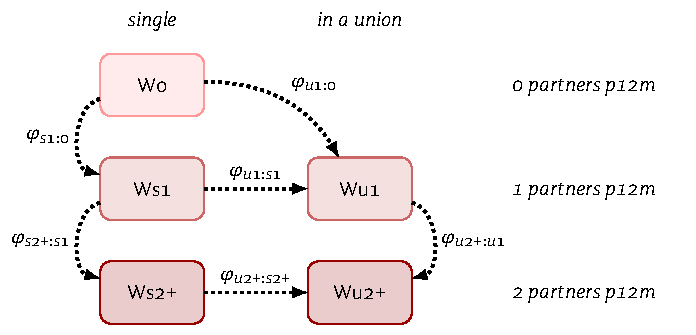
\includegraphics[scale=.8]{diag.nsw.adj}
  \caption{Illustration of how the proportions of women (and equivalently men)
    are adjusted / reallocated between union / partners in p12m strata
    based on odds ratios $\varphi$}
  \label{fig:model.nsw.adj}
  \floatfoot{\raggedright
    p12m: within the past 12 months;
    W0: 0 partners in p12m;
    Ws1: single (not married/cohabiting) and 1 partner in p12m;
    Wu1: in a union (married/cohabiting) and 1 partner in p12m;
    Ws2+: single and 2+ partners in p12m;
    Wu2+: in a union and 2+ partners in p12m.
    $\varphi$: odds of truly being in the second (arrowhead) \vs first (tail) group.}
\end{figure}
%---------------------------------------------------------------------------------------------------
\paragraph{Union Status}
I assumed that under-reporting of main/spousal partnerships was minimal,
but that some ``main'' partnerships may not be captured in
the definition ``married/cohabiting'' from \cite{SDHS2006,SHIMS2};
thus $\varphi_{u1:0}$, $\varphi_{u1:s1}$, and $\varphi_{u2+:s2+}$
would be small but greater than 1
(horizontal transitions in Figure~\ref{fig:model.nsw.adj}).
Moreover, based on the median age of marriage, 23--29 \cite{SDHS2006},
approximately half of respondents aged 15--49 would have been married,
whereas only 28--39\% of women and men reported being in a union
(Figure~\ref{fig:Cwp.2006}~and~\ref{fig:Cwp.2016}),
although some marriages end in divorce/widowing \cite{SDHS2006}.
Thus, I sampled each of $\varphi_{u1:0}$, $\varphi_{u1:s1}$, and $\varphi_{u2+:s2+}$
from $1+\opname{Gamma}(\alpha,\beta=1)$
with $\alpha=.5$ for women and $\alpha=.3$ for men,
yielding mean (95\%~CI): 1.50~(1.00,~3.51) and 1.30~(1.00,~2.90), respectively.
%---------------------------------------------------------------------------------------------------
\paragraph{Partner Numbers}
Next, I defined $\varphi_{s1:0}$, $\varphi_{s2+:s1}$, and $\varphi_{u2+:u1}$ as follows
(vertial transitions in Figure~\ref{fig:model.nsw.adj}).
The median age of first sex in Eswatini was
approximately 18 for women and 19.5 for men \cite{SDHS2006}.
Thus, the 31--36\% of women and 34--41\% of men aged 15--49 reporting no partners in p12m
(Figure~\ref{fig:Cwp.2006}~and~\ref{fig:Cwp.2016}) is likely overestimated,
although some individuals may be abstinent in p12m following sexual debut.
I assumed that women had 3 and men had 2 times the odds of
actually having 1 casual partner in p12m while reporting no partners.
Thus, I sampled $\varphi_{s1:0}$ from $1+\opname{Gamma}(\alpha,\beta=1)$
with $\alpha=2$ for women and $\alpha=1$ for men,
yielding mean (95\%~CI): 3.00~(1.24,~6.57) and 2.00~(1.03,~4.69), respectively.
Drawing on \cite{Behanzin2013}, I assumed that ``single'' women and men (not married/cohabiting)
were less likely to report multiple partners in p12m, but women more so.
Thus, I sampled $\varphi_{s2+:s1}$ from $1+\opname{Gamma}(\alpha,\beta=1)$
with $\alpha=4$ for women and $\alpha=1$ for men,
yielding 5.00~(2.09,~9.77) and 2.00~(1.03,~4.69).
I made a similar assumption about married/cohabiting women and men,
with the same odds for men, but even greater odds of non-reporting among women.
I sampled $\varphi_{u2+:u1}$ from $1+\opname{Gamma}(\alpha,\beta=1)$
with $\alpha=6$ for women and $\alpha=1$ for men,
yielding 7.00~(3.20,~12.67) and 2.00~(1.03,~4.69).
%---------------------------------------------------------------------------------------------------
\subsubsection{Bias Adjustment: Resulting Group Sizes \& Partner Numbers}\label{model.par.nsw.res}
The mean resulting adjusted proportions $W'$ and $M'$
from solving the system with the assumed odds ratios $\varphi$
are illustrated in Figure~\ref{fig:Cwp.adj}, which can be compared to
the reported proportions in \sfref{fig:Cwp.2006}~and~\sfref{fig:Cwp.2016}.
Figure~\ref{fig:Cwp.adj.dens} also illustrates the empiric density distributions
for each element $W'_{i}$ and $M'_{i}$.
Numerically, the mean (95\%~CI) estimates were:
\begin{itemize}
  \item $W'_{0} = 17~(9,~27)$\% of women and $M'_{0} = 25~(13,~35)\%$ of men had 0 partners in p12m
  \item $W'_{1} = 66~(57,~75)$\% of women and $M'_{1} = 49~(37,~61)\%$ of men had 1 partners in p12m
  \item $W'_{2+} = 17~(10,~27)$\% of women and $M'_{2+} = 26~(15,~44)$\% of men had 2+ partners in p12m
  \item $W'_{u1} / W'_{01} = 38~(21,57)$\% women and $M'_{u1} / M'_{01} = 35~(23,~50)$\% men
    with 0--1 partners in p12m were in a main/spousal partnership
  \item $W'_{s1} / W'_{01} = 41~(19,65)$\% women and $M'_{s1} / M'_{01} = 31~(15,~55)$\% men
    with 0--1 partners in p12m were in a single casual partnership
  \item $W'_{u2+} / W'_{2+} = 32~(9,55)$\% women and $M'_{u2+} / M'_{2+} = 38~(13,~62)$\% men
    with 2+ partners in p12m were in a main/spousal partnership,
    and the rest had only casual partnerships.
\end{itemize}
%---------------------------------------------------------------------------------------------------
\paragraph{Group Sizes}
From these results, I defined the sizes of the modelled lower and medium activity groups,
and the average numbers of main/spousal partnerships per person.
I assumed that $W'_{2+}$ and $M'_{2+}$ included FSW and client population sizes, respectively
(see \sref{model.par.sw.size}).
Thus, the populations size of medium activity women was defined as
$P_{s_{1}i_{2}} = W'_{2+} - P_{s_{1}i_{34}}$.
Sampling $W'_{2+}$ from a BAB distribution with 95\%~CI (10,~27)\%,
the resulting 95\%~CI for medium activity women $P_{s_{1}i_{2}}$ was (6,~25)\% of women.
The lowest activity women population size was then defined as $1 - P_{s_{1}i_{234}}$,
representing (73,~90)\% of women.
Since there is greater uncertainty in the client population size,
the same approach for the medium activity men population size $P_{s_{2}i_{2}}$
could yield negative values.
Instead, I sampled $P_{s_{2}i_{2}}$ directly from
a BAB distribution with 95\%~CI (10,~17)\%, yielding
95\%~CI for $P_{s_{2}i_{234}}$ of (15,~50)\% of men,
which is close to (15,~44)\% from $M_{2+}$.
The lowest activity men were then then defined as $1 - P_{s_{2}i_{234}}$,
representing (50,~85)\% of men.
%---------------------------------------------------------------------------------------------------
\paragraph{Main/Spousal Partnerships}
To simplify model fitting, I sampled a common proportion of
individuals reporting a main/spousal partnership from a BAB distribution with 95\%~CI (25,~50)\%,
applied to all women and men in the lowest activity groups ($C_{p_{1}s_{12}i_{1}}$),
as well as all women in the median activity group ($C_{p_{1}s_{1}i_{2}}$).
Then, \eqrefs{eq:C2Q}{eq:C2K} were used to define $Q$ and $K$, respectively.
Since FSW and clients had fewer main/spousal partnerships (see \sref{model.par.nsw.sw}),
I calculated the proportion of men in the medium activity group having main/spousal partnerships
$K_{p_{1}s_{2}i_{2}}$ to balance the total number of main/spousal partnerships among women and men.
%---------------------------------------------------------------------------------------------------
\paragraph{Casual Partnerships}
I similarly defined a common proportion of women and men in the lowest activity groups
reporting casual partnership $C_{p_{2}s_{12}i_{1}}$ with 95\%~CI (20,~55)\%.
However, the number of casual partnerships among $W_{2+}$ and $M_{2+}$ ramains uncertain.
The analysis above provides no information on these values,
but the number of partners in p12m for the medium activity groups must be at least about 1.5
to ensure these women and men actually have 2+ partners in p12m.
Thus, I sampled the number of casual partners reported by women in the medium activity group
$C_{p_{2}s_{1}i_{2}}$ from a gamma distribution with 95\%~CI (1.2,~2),
and computed $Q$ and $K$ via \eqrefs{eq:C2Q}{eq:C2K}.
As before, I calculated the numbers of casual partnerships among men in the medium activity group
$K_{p_{2}s_{2}i_{2}}$ to balance total casual partnerships.
%---------------------------------------------------------------------------------------------------
\subsubsection{Main/Spousal \& Casual Partnerships among FSW \& Clients}\label{model.par.nsw.sw}
Among Swati FSW, the mean number of total non-paying partners in the past month was
approximately 1--1.5 (Table~\ref{tab:fsw.ratios}),
which may include both main/spousal partners and casual partners.
Among FSW in South Africa \cite{Wells2018} and Kenya \cite{Voeten2007},
while 54 and 72\% (respectively) reported being in a relationship, only 6 and 3\% were married,
although many non-marital partners may still constitute effectively ``main'' partnerships
with respect to condom use and duration.
Thus, I assumed that:
50\% of all FSW reported a main/spousal partner (\ie $C_{p_{1}s_{1}i_{34}} = 0.5$);
lower risk FSW reported $C_{p_{2}s_{1}i_{3}} = 0.5$ casual partners; and
higher risk FSW reported $C_{p_{2}s_{1}i_{4}} = 1.0$ casual partners, on average.
\par
Available data suggest that about half of clients also report non-sex work partners,
which are not always distinguished as main/spousal \vs casual partnerships
\cite{Lowndes2000,Santo2005}.
Non-paying partners of FSW are also often clients of other FSW \cite{Voeten2007,Godin2008}.
Yet, clients of FSW also tend to be younger and more likely to be
never/formerly married \vs non-client men \cite{Lowndes2000,Carael2006}.
So, I assumed that clients reported
half the numbers of main/spousal partnerships compared to lowest activity men:
$C_{p_{1}s_{2}i_{34}} = 0.5\,C_{p_{1}s_{2}i_{1}}$, and
25--100\% the numbers of casual partnerships compared to medium activity women (uniform prior).
As before, I computed $Q$ and $K$ via \eqrefs{eq:C2Q}{eq:C2K}.
